\section{Modelling} \label{sec:mod} % Incl. Subsection "Component Models"
The purpose of this chapter is to outline the linear model of the system. The model is intended to be used as a state-space control model for rotor speed control and fore-aft motion damping. The fore-aft motion dynamics of floating wind turbines are slow (a period of 30 seconds is normal) and the modelling is approached with this in mind: Dynamics which are relatively fast compared to the fore-aft motion dynamics are not included since they are of little importance to the control objective. Examples of such dynamics include but are not limited to: Blade, drivetrain and converter dynamics. Instead such components models are either completely left out or modelled with algebraic equations. 


%\subsection{wtLin component models} \label{sec:compcomps}
%\sout{A Matlab tool named wtLin has been developed by the LaC department in Vestas for creating linear models of their turbines based on simple component models and parameters extracted from VTS parts files. The tool's component models can be connected in loops based on the input-output variables of each component model in a manner chosen by the user. A component can be in the form of a physical system such as a generator or a converter but can also be models of physics which are relevant for the system such as the interaction between the tower movement and the free wind.
%
%The tool takes as input an operating point and a specific set of components. It outputs a connected linear state-space model at that operating point.
%


\subsection{Component models} \label{sec:comp}
A component approach to modelling is adopted where system parts are modelled individually. Each component takes a set of inputs and calculates a set of outputs. If the components contain dynamics they include internal states. Non-linear components are linearised individually at an operating point (OP). Model parameters and OPs are extracted from Vestas Turbine Simulator (VTS) with a tool developed by the LaC department called wtLin which also contains all the model components. When the components are defined in the correct manner the Matlab \textit{connect()} function can used to create a connected model.

\smallskip
\noindent In this section the relevant component models are derived. The modelled components are:
\begin{itemize}
	\item Drivetrain
	\item Generator
	%\item Converter
	\item Aerodynamic torque
	\item Aerodynamic thrust
	\item Rotor wind
	\item Tower fore-aft motion
	\item Pitch system
	\item Full load controller
\end{itemize}
In \cref{sec:comp_connected} the components are connected such that the flow of information in the model is apparent. 


\subsubsection{Drivetrain} \label{sec:comp_drv}
As mentioned in \cref{sec:intro_wtcomponents} the drivetrain connects the rotor with the generator through a gearbox. In a simple \textit{stiff} drivetrain model, dampening and spring effects are left out. Thus when a torque is applied at the rotor resulting in a change in twist angle at the rotor the resulting twist angle at the generator is instant and directly proportional to the twist angle at the rotor. In the appendix in \cref{sec:mod_drt_flex} a model of a flexible drivetrain can be found. Due to the relatively fast dynamics of the drivetrain in relation to the WT eigenfrequency these dynamics can be left out. 

The stiff drivetrain consists of two free inertias connected through a gearbox. The drivetrain is modelled from newtons second law for rotation like so:
\begin{equation}\label{eq:wtlin_comp_drivetrain}
	(J_{gL} + J_{r}) \ddot{\theta}_r = T_{r} + T_{g}
\end{equation}
where the $ g $ and $ r $ subscripts denote the generator-side and rotor-side intertias ($ J $), torques ($ T $) and angles ($ \theta $).
The torques are related to the low-speed rotor side and thus the high-speed generator side inertias are mapped to the low speed side:
\begin{equation} \label{eq:wtlin_comp_inertiamap}
	J_{gL} = J_{g} \left(\dfrac{N_r}{N_g}\right)^2
\end{equation}
where $ N_r $ and $ N_g $ is the number of teeth on the rotor and generator side of the gearbox respectively. The rotor spins at angular velocity $ \dot{\theta}_r = \Omega $.

Given $ \dot{\Omega} = \ddot{\theta}_r $ and isolating the rotor speed rate of change the model becomes:
\begin{equation}\label{key}
	 \dot{\Omega} = \dfrac{T_{r} + T_{g}}{\left(\dfrac{N_r}{N_g}\right)^2 J_{g} + J_{r}}
\end{equation}

The component inputs are $ \{T_r, T_g\} $ and the output is $ \{\Omega\} $ 



\subsubsection{Generator} \label{sec:comp_generator}
The generator is mechanically connected to the drivetrain and is electrically connected to the converter. It is used to control the rotor speed during PLC by means of the generator torque. 

While the generator model in wtLin includes the generator efficiencies they are left out here for simplicity. In the appendix in \cref{sec:comp_generator_eff} the generator model is derived including efficiencies. No generator dynamics are modelled and thus the model simply consists of algebraic equations.

The power of a rotating machine can be defined as the product of torque and rotational velocity:
\begin{equation}\label{eq:comp_power_in_rot}
	P_{g} = T_g \omega
\end{equation}
The non linear generator model is then defined by rearranging \cref{eq:comp_power_in_rot}:
\begin{equation}\label{eq:comp_gen_torque}
	T_g(P_g, \omega) = \dfrac{P_g}{\omega}
\end{equation}
The linear model of the generator is obtained through a taylor expansion. \cref{eq:comp_power_in_rot} is an algebraic equation describing the absolute value of the generator torque and not its rate of change as it would have been for a model including dynamics. Therefore the taylor expansion linearisation at the OP yields an affine linear approximation at the OP:
\begin{equation}\label{eq:comp_gen_taylor}
	T_g( P_g, \omega) \approx T_g(P_{g_o}, \omega_o) + 
	\left. \dfrac{\partial T_g( P_g, \omega)}{\partial P_g} \right |_{P_{g_o},\omega_o} ( P_g-P_{g_o}) + 
	\left. \dfrac{\partial T_g( P_g, \omega)}{\partial \omega} \right |_{P_{g_o},\omega_o} (\omega - \omega_o)
\end{equation}
Below the the generator torque sensitivity to the grid power change term from \cref{eq:comp_gen_taylor} is derived.
\begin{equation} 
	\dfrac{\partial T_g( P_g, \omega)}{\partial P_g} = \dfrac{\partial \left (\dfrac{P_g}{\omega}\right )}{\partial P_g} \label{eq:comp_gen_1} = \dfrac{1}{\omega}
\end{equation}
The generator torque sensitivity to rotational velocity change from \cref{eq:comp_gen_taylor} is then derived:
\begin{align}
	\dfrac{\partial T_g(P_g, \omega)}{\partial \omega} & = \dfrac{\partial \left (\dfrac{P_g}{\omega}\right )}{\partial \omega} \\
	& = P_g \dfrac{\partial \left (\dfrac{1}{\omega}\right )}{\partial \omega} \\
	& = -P_g \, \dfrac{1}{\omega^2}
\end{align}
The generator model derived above is referred to the rotor side by replacing $ \omega $ with $ \Omega $ where $ \Omega = \left (\frac{N_r}{N_g} \right ) \omega $. This yields the affine linear generator model evaluated at the OP $ (P_{g_o}, \Omega_o) $:
\begin{equation}
	T_g(P_g, \Omega) \approx \dfrac{P_{g_o}}{\omega_o} + \left. \dfrac{1}{\dfrac{N_g}{N_r} \Omega} \right |_{P_{g_o},\Omega_o} (P_g - P_{g_o}) \\ 
	\left. - P_g \, \dfrac{1}{\left( \dfrac{N_g}{N_r} \Omega \right)^2} \right |_{P_{g_o},\Omega_o} (\Omega - \Omega_o)
\end{equation}
The goal is to have a linear model of the generator around an OP and therefore the change in the generator torque from the OP is defined:
\begin{equation}
	\hat T_g(P_g, \Omega) \approx \left. \dfrac{1}{\dfrac{N_g}{N_r} \Omega} \right |_{P_{g_o},\Omega_o} (P_g - P_{g_o}) \\ 
	\left. - P_g \, \dfrac{1}{\left( \dfrac{N_g}{N_r} \Omega \right)^2} \right |_{P_{g_o},\Omega_o} (\Omega - \Omega_o)
\end{equation}
where $ \hat T_g = T_g - T_{g_o} $.

When the model is linearised in a FLC operating point, P is constant and therefore the first term in the above equation is also zero. The second term is the \textit{negative damping} term which yields and increase in the generator torque when the rotational speed decreases which even further decreases the rotational speed.

The component model inputs are $ \{P, \Omega\} $ and the output is $ \{T_g\} $


%\subsubsection{Converter} \label{sec:comp_conv_unity}
%The converter connects the generator with the grid and it is controlled by the power controller. It handles the power flow from the generator to the grid.
%
%The dynamics of modern converters are much faster than the rotor and tower dynamics and therefore it is simply modelled as an algebraic equation as a direct feed-through:
%\begin{equation}\label{eq:comp_convdft}
%	P_{conv} = P_{ref}
%\end{equation}
%In other words the converter is treated as a \textit{black box} system which, when given a power reference, delivers a power equal to said power reference instantly. 
%
%The input is $ \{P_{conv}\} $ and the output is $ \{P_{ref}\} $


\subsubsection{Aerodynamic torque} \label{sec:comp_aero_torque}
In \cref{sec:theory_fowt_challenges} it was explained that it was convenient to use the pre-calculated thrust coefficient values $ C_T $ to determine the stationary thrust. Likewise pre-calculated power coefficient tables $ C_p $ can be used to calculate the stationary torque. Both $ C_p $ and $ C_T $ are extracted and linearised at the OP with wtLin.

In \cref{eq:power_w_Cp} the extractable power from the free wind was defined. When combining this equation with the definition of power in a mechanical system the torque on the rotor can be expressed:
\begin{equation}\label{eq:comp_Mrot_lambda}
	T_r(\Omega, \lambda) = \dfrac{1}{2} \rho A_d v^3 \, C_p(\theta, \lambda) \dfrac{1}{\Omega}
\end{equation}
The TSR is dependent on $ \Omega $ and $ v $ and thus the rotor torque model ends up being dependent on $ \theta $, $ \Omega $ and $ v $:
\begin{equation}\label{eq:comp_Mrot_wind}
	T_r(\theta, \Omega, v) = \dfrac{1}{2} \rho A_d v^3 \, C_p(\theta, \Omega, v) \dfrac{1}{\Omega}
\end{equation}
The model is linearised at an OP with a taylor expansion $ (\theta_o, \Omega_o, v_o) $:
\begin{align}
	T_r(\theta, \Omega, v) \approx T_r(\theta_o, \Omega_o, v_o) 
	& + \left. \dfrac{\partial T_r(\theta, \Omega, v)}{\partial \theta} \right |_{\theta_o, \Omega_o, v_o} ( \theta-\theta_o) \\
	& + \left. \dfrac{\partial T_r(\theta, \Omega, v)}{\partial \Omega} \right |_{\theta_o, \Omega_o, v_o} ( \Omega-\Omega_o) \\
	& + \left. \dfrac{\partial T_r(\theta, \Omega, v)}{\partial v} \right |_{\theta_o, \Omega_o, v_o} ( v - v_o)
\end{align}
The derivation of the linear model is excluded in the report for this and the following components since the concept of linearising through a taylor expansion of a component model was demonstrated in the \hyperref[sec:comp_generator]{\textbf{generator component model section}}. Retrieving a linear model can easily be done for the remainder of the components with the \textit{jacobian()} Matlab function.

The component inputs are $ \{\theta, \Omega, v\} $ and the output is $ \{T_r\} $

\subsubsection{Aerodynamic thrust} \label{sec:comp_aero_thrust}
The stationary rotor thrust force $ F_T $ is calculated from the pre-calculated thrust table $ C_T $ yielding the model:
\begin{equation} \label{eq:comp_aero_thrust}
	F_T(\theta, \Omega, v) = \dfrac{1}{2} \rho A_d v^2 C_T(\theta, \Omega, v)
\end{equation}
$ C_T $ is a mapping from the pitch angle, rotor velocity and wind speed to a total stationary rotor thrust. The model is linearised with a taylor expansion.

The component inputs are $ \{\theta, \Omega, v \} $ and the output is $ \{F_T\} $


\subsubsection{Rotor wind} \label{sec:comp_rot_wind}
There is an interaction between the tower fore-aft movement and the wind speed which ultimately results in a constantly changing wind speed as seen from the rotor's point of view. Thus it is necessary to calculate the \textit{free} wind speed as observed from the rotors point of reference. This is simply done by subtracting the translational velocity in the  \textbf{y} direction $ v_y $ from the free wind speed $ v_0 $. Note that the \textbf{x} and \textbf{y} directions are interchanged in the Vestas notation of the floating degrees of freedom in relation to the notation used in most literature. This is further touched upon in the following section. 
\begin{equation}\label{eq:comp_rotorwind}
	v_{0_{rot}} = v_{0} - v_y
\end{equation}
$ v_{0_{rot}} $ is \underline{not} the rotor wind (which is the wind speed at the rotor plane) but the free wind modified by the turbine velocity.

The component inputs are $ \{v_0, v_y\} $ and the output is $ \{v_{0_{rot}}\} $


\subsubsection{Tower fore-aft motion} \label{sec:comp_foreaft_mod}
The fore-aft motion is both the \textit{surge} and \textit{pitch} motion of turbine structure. In most literature the degree of fredom notation follows the convention in \cref{fig:fowt_coordinates}. Vestas uses a slightly different notation where \textbf{x} and \textbf{y} are interchanged such that for the Vestas notation y is in the \textit{surge} direction and x in the \textit{sway} direction and \textit{pitch} is called \textit{tilt}. This report for the most part follows the notation in \cref{fig:fowt_coordinates}. Since Vestas and the wtLin tool adopts the Vestas notation the equations presented make use of this notation instead.
\begin{figure}[ht]
	\centering
	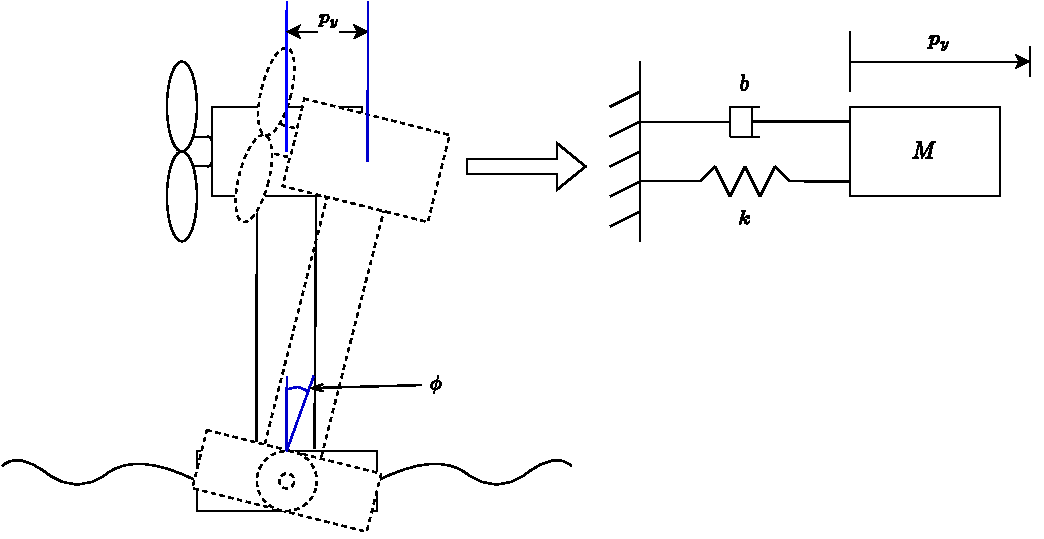
\includegraphics[width=0.9\linewidth]{Graphics/wtLinForeAftMotionModel.pdf}
	\caption{Illustration of the mass spring damper approximation of the fore-aft tower movement.}
	\label{fig:wtLin_fore-aft_diagram}
\end{figure}

The fore-aft motion is modelled by a mass-spring-damper system whose movement is defined to be at nacelle height. This choice is initially made because a sensor in VTS is currently located at nacelle height which is utilized by the FATD controller. For simplicity it is assumed that the foundation does not translate in any direction and therefore the translation at nacelle height is due to the pitching $ \phi $ of the structure. An illustration of this is seen in \cref{fig:wtLin_fore-aft_diagram}. This is obviously a heavily simplified model. It assumes a stiff nacelle-tower-foundation structure and the stability and dynamics from the hydrodynamic, buoyancy, ballast and mooring line forces are approximated into the mass, spring and damper coefficients. Furthermore the mass $ m $ represents the inertia of the structure pitching. The governing equations for the mass-spring-damper system are:
\begin{equation}\label{eq:comp_fore-aft_ay1}
	\ddot{p}_y m = F_{rot} - F_d + F_s
\end{equation}
where $ p_y $ is the pitch equivalent translation position in the surge direction, $ F_{rot} $ is the rotor force and $ F_d $ and $ F_s $ are the damper and spring forces respectively.

when isolating $ \ddot{p}_y $ and expanding $ F_d $ and $ F_s $, \cref{eq:comp_fore-aft_ay1} becomes:
\begin{equation}\label{eq:comp_fore-aft_ay2}
	\ddot{p}_y = \dfrac{F_{rot} - b \dot{p}_y - k p_y}{m}
\end{equation}
where $ b $ and $ k $ are the damper and spring coefficients respectively.

We then define:
\begin{align}
	\dot{v}_y & = \ddot{p}_y \label{eq:comp_fore-aft_ay} \\
	\dot{p}_y & = v_y \label{eq:comp_fore-aft_vy}
\end{align}
which yields the fore-aft tower model:
\begin{align}
	\dot{v}_y & = \dfrac{F_{rot} - b v_y - k p_y}{m}  \label{eq:comp_fore-aft_1} \\
	\dot{p}_y & = v_y \label{eq:comp_fore-aft_2}
\end{align}
Furthermore the fore-aft tower model transfer function from rotor thrust $ F_{rot} $ to equivalent surge translation $ p_y $ can be written on the standard second order transfer function form (seen in \cref{eq:std_tf}) in the laplace domain as seen below:
\begin{equation}\label{eq:comp_fore_aft_tf}
	\dfrac{p_y}{F_{rot}} = \dfrac{\dfrac{1}{m}}{s^2 + \dfrac{b}{m} s + \dfrac{k}{m}}
\end{equation}
From comparison to the standard TF it can be derived that:
\begin{align}
	k & = (2 \pi f_{eig})^2 m \label{eq:comp_fore_aft_tf_k} \\
	b & = 2 \zeta \sqrt{k m} \label{eq:comp_fore_aft_tf_b}
\end{align}
where $ f_{eig} $ represents the natural frequency of the system while $ \zeta $ is the damping factor. 

This leaves three new tuning parameters to be considered: $ m $, $ f_{eig} $ and $ \zeta $. Since this simple model is a crude approximation of a much more complex system these parameters can not be directly inferred from any inputs or parameters in VTS. They need to be tuned such that the response of the model fits the real system as close as possible. In the appendix in \cref{sec:app_mod_foreaft_fitting} this process is further described in detail.

\medskip
The second order TF standard form:
\begin{equation}\label{eq:std_tf}
	T(s) = \dfrac{\omega_n^2}{s^2 + 2 \zeta \omega_n s + \omega_n^2}
\end{equation}

The component input is $ \{F_{rot} \} $ and the output is $ \{p_y, v_y\} $


\subsubsection{Pitch system} \label{sec:comp_pitch}
The pitch system consists of both the local pitch controller and the hydraulic and electrical parts. The pitch controller takes the pitch reference $ \theta_{ref} $ as input and outputs a voltage in a range which through the electrical and mechanical system translates to a pitch position. 

While the pitch system dynamics can be assumed to be fast enough with regards to the control objective to be left out. Therefore the pitch system is simply modelled as a direct feed-through. Alternatively the pitch system could have been approximated with a single order low-pass filter as it's done in the appendix in \cref{sec:comp_pitch_dyn}. 
\begin{equation}\label{eq:comp_pitch_freq}
	\theta = \theta_{ref}
\end{equation}
The component input is $ \{\theta_{ref}\} $ and the output is $ \{\theta \} $


\subsubsection{Full load controller} \label{sec:comp_flc}
The FLC is a PI controller on the form seen in \cref{fig:PIcontroller}. The output of the FLC is the pitch reference $ \theta_{ref} $ which is added with the FATD pitch reference contribution $ \theta_{FATD} $ if the FATD is active. The controller to be developed in this project acts as both the FLC and FATD. Therefore this FLC component is only included in the model to see how the linear turbine model behaves under normal operation.
\begin{figure}[ht]
	\centering
	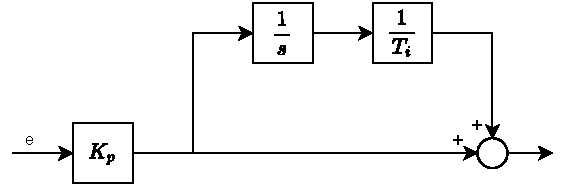
\includegraphics[width=0.5\linewidth]{Graphics/PiController.pdf}
	\caption{Block diagram of the PI controller on the \textit{$T_i$} form.}
	\label{fig:PIcontroller}
\end{figure}
When including the sensitivity gain scheduling the laplace domain controller is therefore:
\begin{equation}\label{eq:comp_flc}
	\theta_{ref}(s) = K_{gs,dP/d\theta} (K_{p, \theta} + K_{p, \theta} \dfrac{1}{T_{i, \theta} s}) e(s)
\end{equation}
%The time domain FLC controller is derived:
%\begin{align}
%	\theta_{ref}(s) & = K_{gs,dP/d\theta} K_{p, \theta} \dfrac{T_{i, \theta} s + 1}{T_{i, \theta} s} e(s) \\
%	\theta_{ref}(s) & = K_{gs,dP/d\theta} K_{p, \theta} (\dfrac{T_{i, \theta} s}{T_{i, \theta} s} + \dfrac{1}{T_{i, \theta} s}) e(s) \\
%	\theta_{ref}(s) & = K_{gs,dP/d\theta} K_{p, \theta} e(s) +  K_{gs,dP/d\theta} K_{p, \theta} \dfrac{1}{T_{i, \theta} s} e(s) \\
%	\theta_{ref}(s) s & = K_{gs,dP/d\theta} K_{p, \theta} e(s) s +  K_{gs,dP/d\theta} K_{p, \theta} \dfrac{1}{T_{i, \theta}} e(s)
%\end{align}
The time domain model can be derived by rearranging and taking the inverse laplace transform which yields:
\begin{equation}\label{eq:comp_flc_time}
	\dot{\theta}_{ref} = K_{gs,dP/d\theta} (K_{p, \theta} \dot{e} + K_{p, \theta} \dfrac{1}{T_{i, \theta}} e)
\end{equation}
The controller parameters are extracted from VTS.

The component input is $ \{e \} $ and the output is $ \{\theta_{ref} \} $


%\subsubsection{Partial Load Controller (PLC)} \label{sec:comp_plc}
%The PLC is a PI-controller on the same form as the \hyperref[sec:comp_flc]{\textbf{FLC}} controller:
%\begin{equation}\label{eq:comp_plc}
%	P_{ref}(s) = K_{gs} (K_{p, P} + K_{p, P} \dfrac{1}{T_{i, P} s}) e(s)
%\end{equation}
%
%Which likewise in the time domain is:
%\begin{equation}\label{eq:comp_plc_time}
%	\dot{P}_{ref} = K_{gs P} K_{p, P} \dot{e} +  K_{gs P} K_{p, P} \dfrac{1}{T_{i, P}}e
%\end{equation}
%
%The component inputs are $ \{e \} $ and the outputs are $ \{P_{ref} \} $


\subsection{The connected model} \label{sec:comp_connected}
In the previous section all individual component models were defined and the non-linear models were linearised at an OP. When the components are connected we are left with a system which is only a function of states and inputs. We can then set up a continuous linear state-space system on the following form:
\begin{equation}\label{eq:state-space-sys}
	\begin{split}
		\dot x &= A x + B u + B_d d \\
		y &= Cx
	\end{split}
\end{equation}
Where $ \dot x $ is the time derivative of the state vector, $ u $ the input vector and $ d $ the disturbance vector with $ x \in R^n $, $ u \in R^m $ and $ u \in R^q $ where $ n $ is the number of states, $ m $ the number of controlled inputs and $ q $ the number of disturbances. A distinction is made between $ u $ and $ d $ because $ u $ represents the controllable inputs which will eventually be the output of the designed controller while $ d $ are uncontrollable inputs such as the wind which affect the system beyond our control. Achieving a system model on this form is necessary for conventional linear state-space controller design.

In \cref{fig:connected_components} a diagram of the connected model can be found. The outputs of most component models can be observed entering adjacent components. The inputs to the full system can be observed to be the rotor speed reference $ wRef $ and the free wind speed $ vfree $. It should be highlighted again that the system contains the FLC controller component described in \cref{sec:comp_flc} which like the other components is embedded in the $ A $ and $ B $ matrices, essentially making it a closed-loop system. When the controller is made in \cref{sec:ctrl-design} the FLC is removed such that the designed controller regulates both rotor speed and the turbine tower top movement.

Outputs are defined from the available sensors in VTS and if the outputs are equal to the states then the output matrix $ C $ only contains ones and zeros.

\begin{figure}[ht]
	\centering
	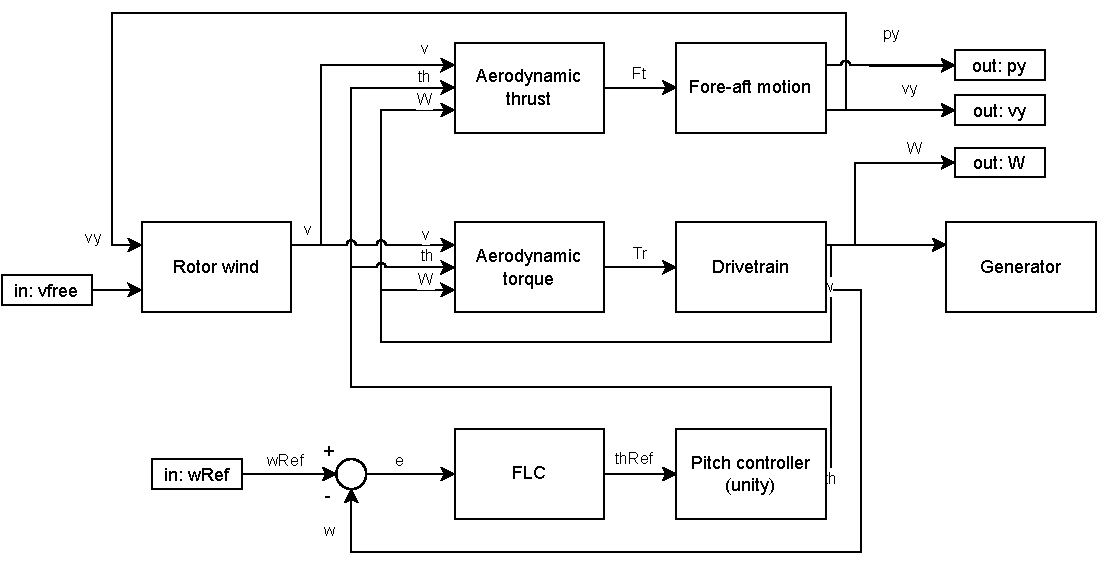
\includegraphics[width=0.99\linewidth]{Graphics/wtLinComponents.pdf}
	\caption{Diagram showing the connections of the components}
	\label{fig:connected_components}
\end{figure}

\subsubsection{Evaluation of model fit} \label{sec:lin_fit_eval}
In the tower fore-aft motion component section in \cref{sec:comp_foreaft_mod} it was explained that a fitting process was necessary to find the parameters which gave the best fit of the linear model. In the appendix in \cref{sec:app_mod_foreaft_fitting} all results from said process are presented and a few of the results are also shown here in \cref{fig:wref-vy_16}. In \cref{fig:sysid_wref-vy_16} the frequency response from VTS is seen. It is generated by applying a test sine to the pitch reference at different frequencies. While the input to the model is the rotor speed reference (due to the FLC PI controller) the test sine is put on the pitch reference for the evaluation. This is because the controller to be developed regulates the pitch reference and thus the response from the pitch reference is of greater interest than from the rotor speed reference. 

The frequency response is plotted from the pitch reference to the surge direction velocity at nacelle height. In \cref{fig:wtlin_wref-vy_16} a bode plot of the linear model is seen from the pitch reference to the surge direction velocity. Black lines are plotted in the linear model bode plot to aid in assessing the fit accuracy. The intersection of the lines are located at the peak of the magnitude of the VTS plot. In the phase plot they are located right before and after the sharp dip in the phase. It is observed that the magnitude of the linear model is around 5-6 dB lower than the VTS model. The phase is furthermore observed almost passing through the cross sections of the black lines. While the fit is not perfect it is deemed good enough to be used for a control model.
\begin{figure*}[ht]
	\centering
	
	\subfloat[VTS frequency response]{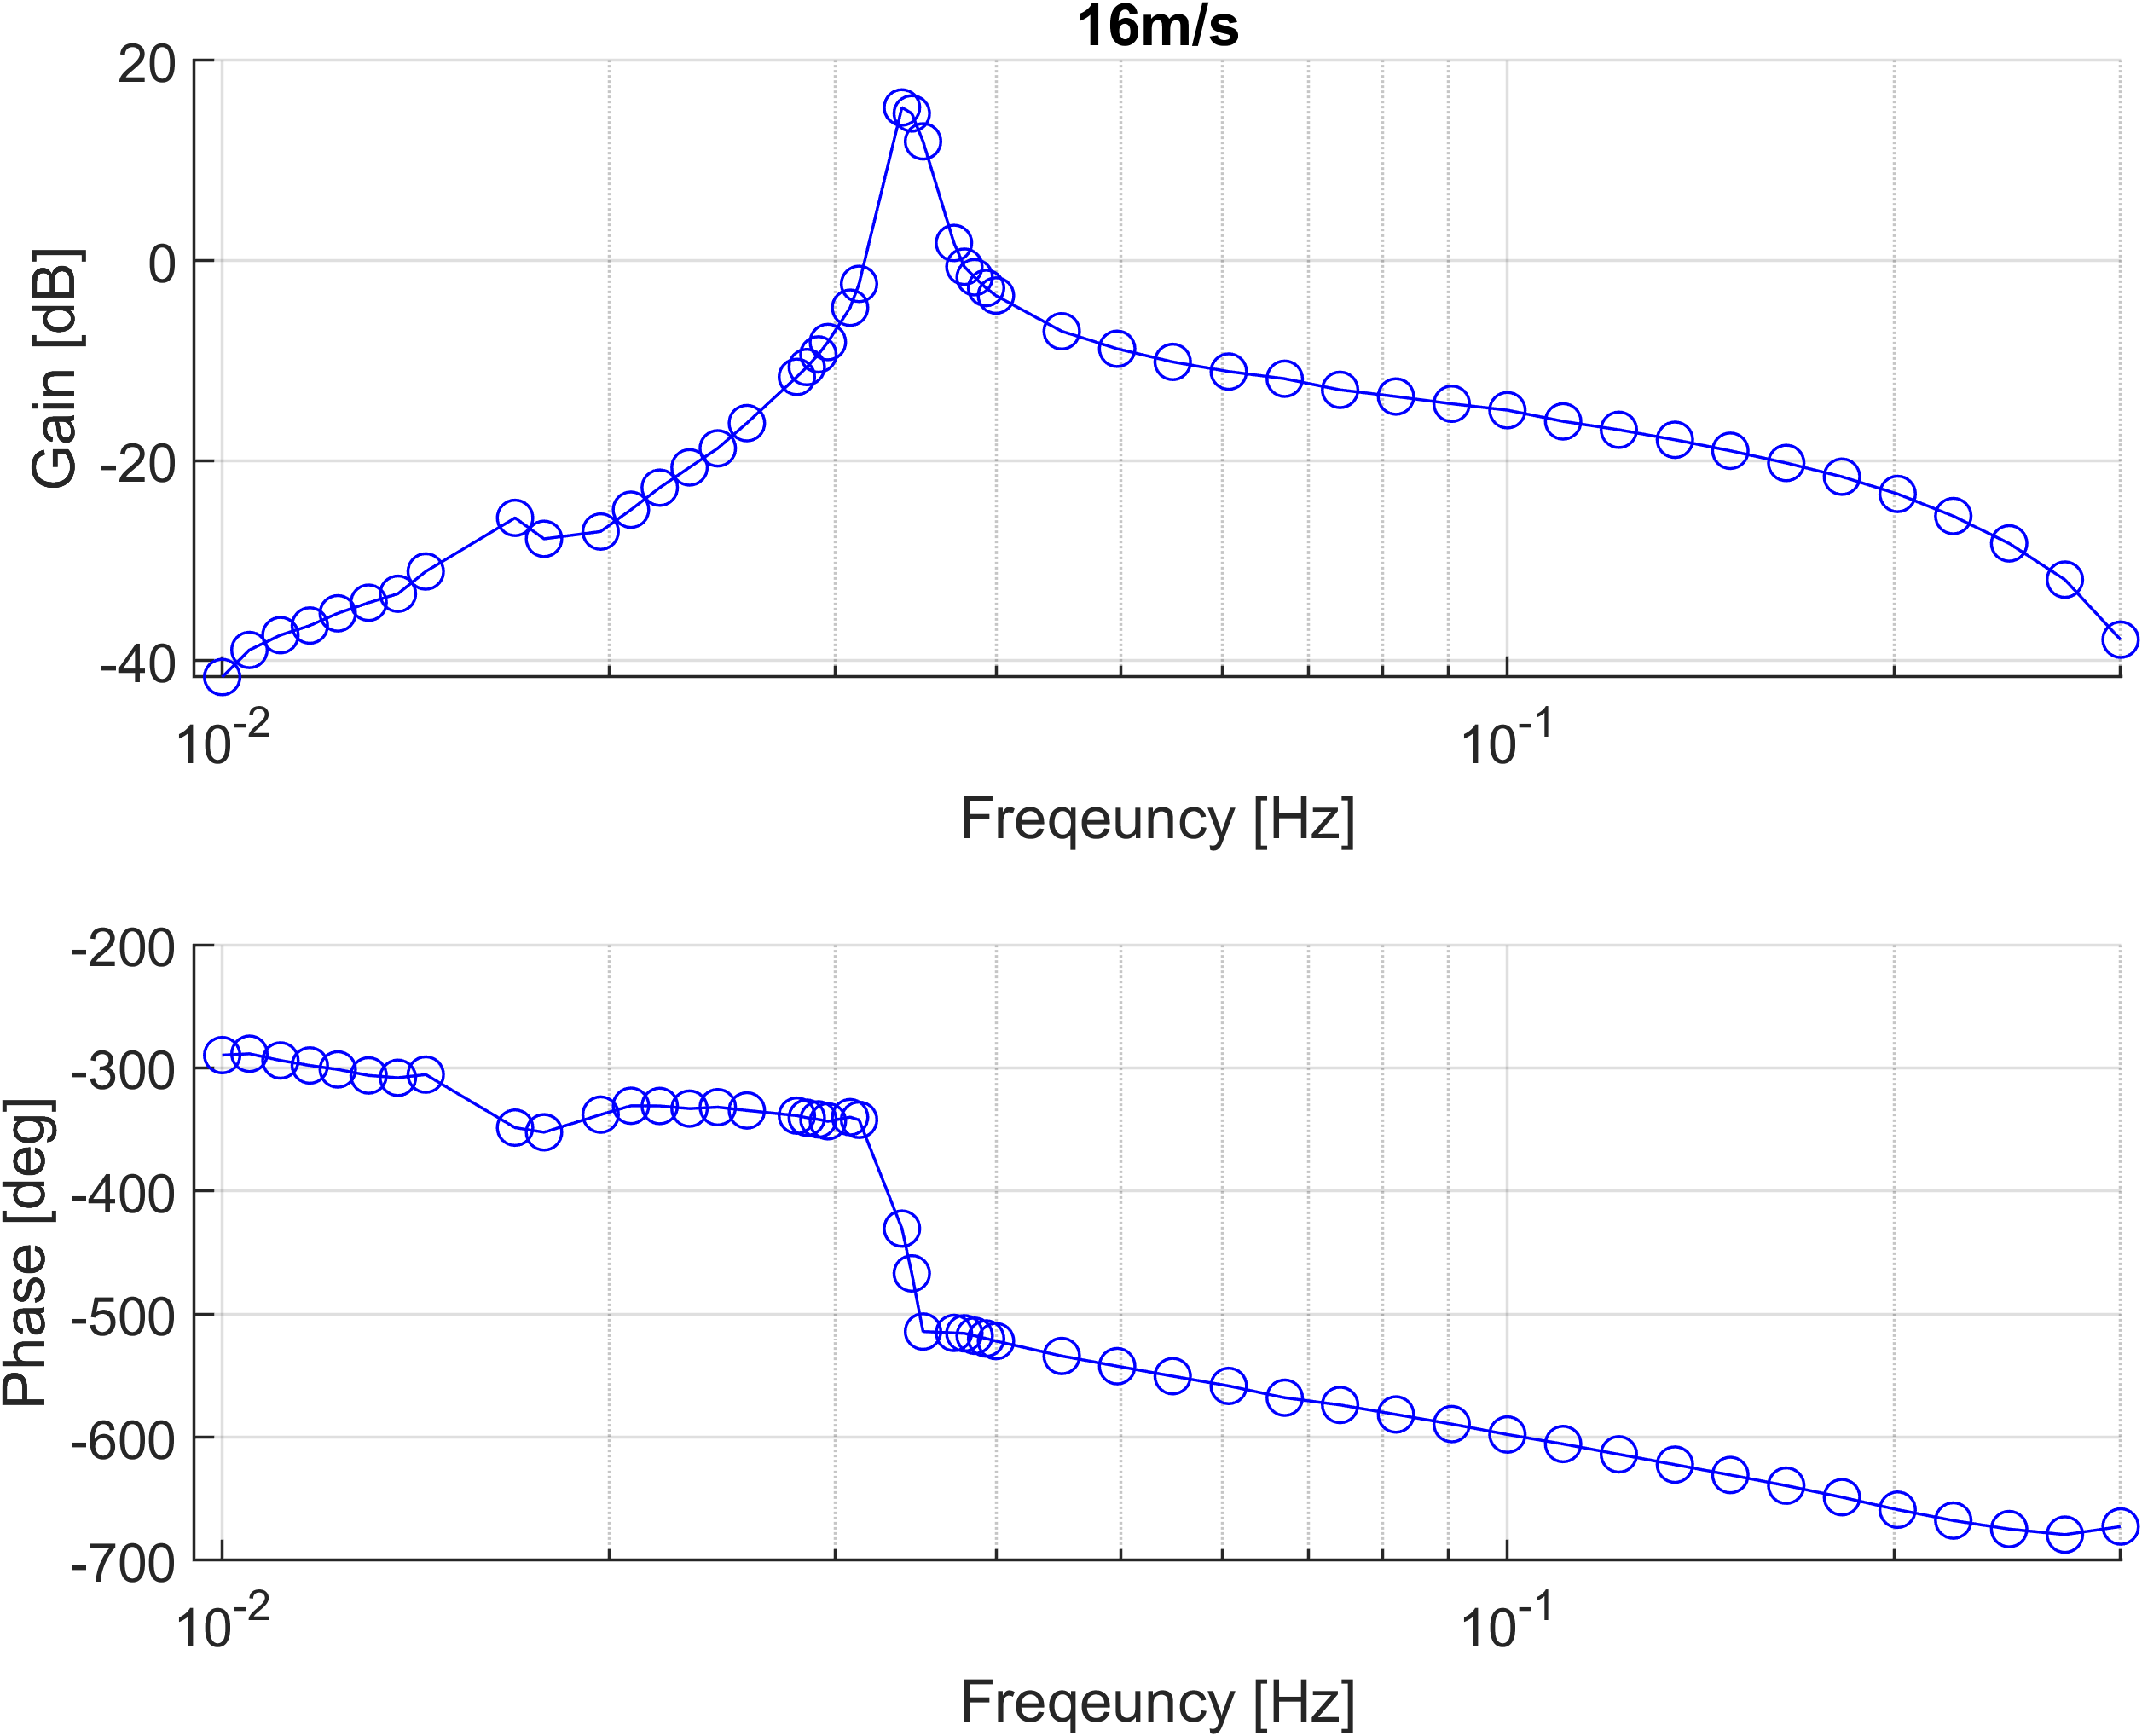
\includegraphics[width=.49\textwidth]{Graphics/TestResults/foreaftFitting/sysid_thSine-vy_16ms.png}
		\label{fig:sysid_wref-vy_16}}
	\hfil
	\subfloat[Linear model response]{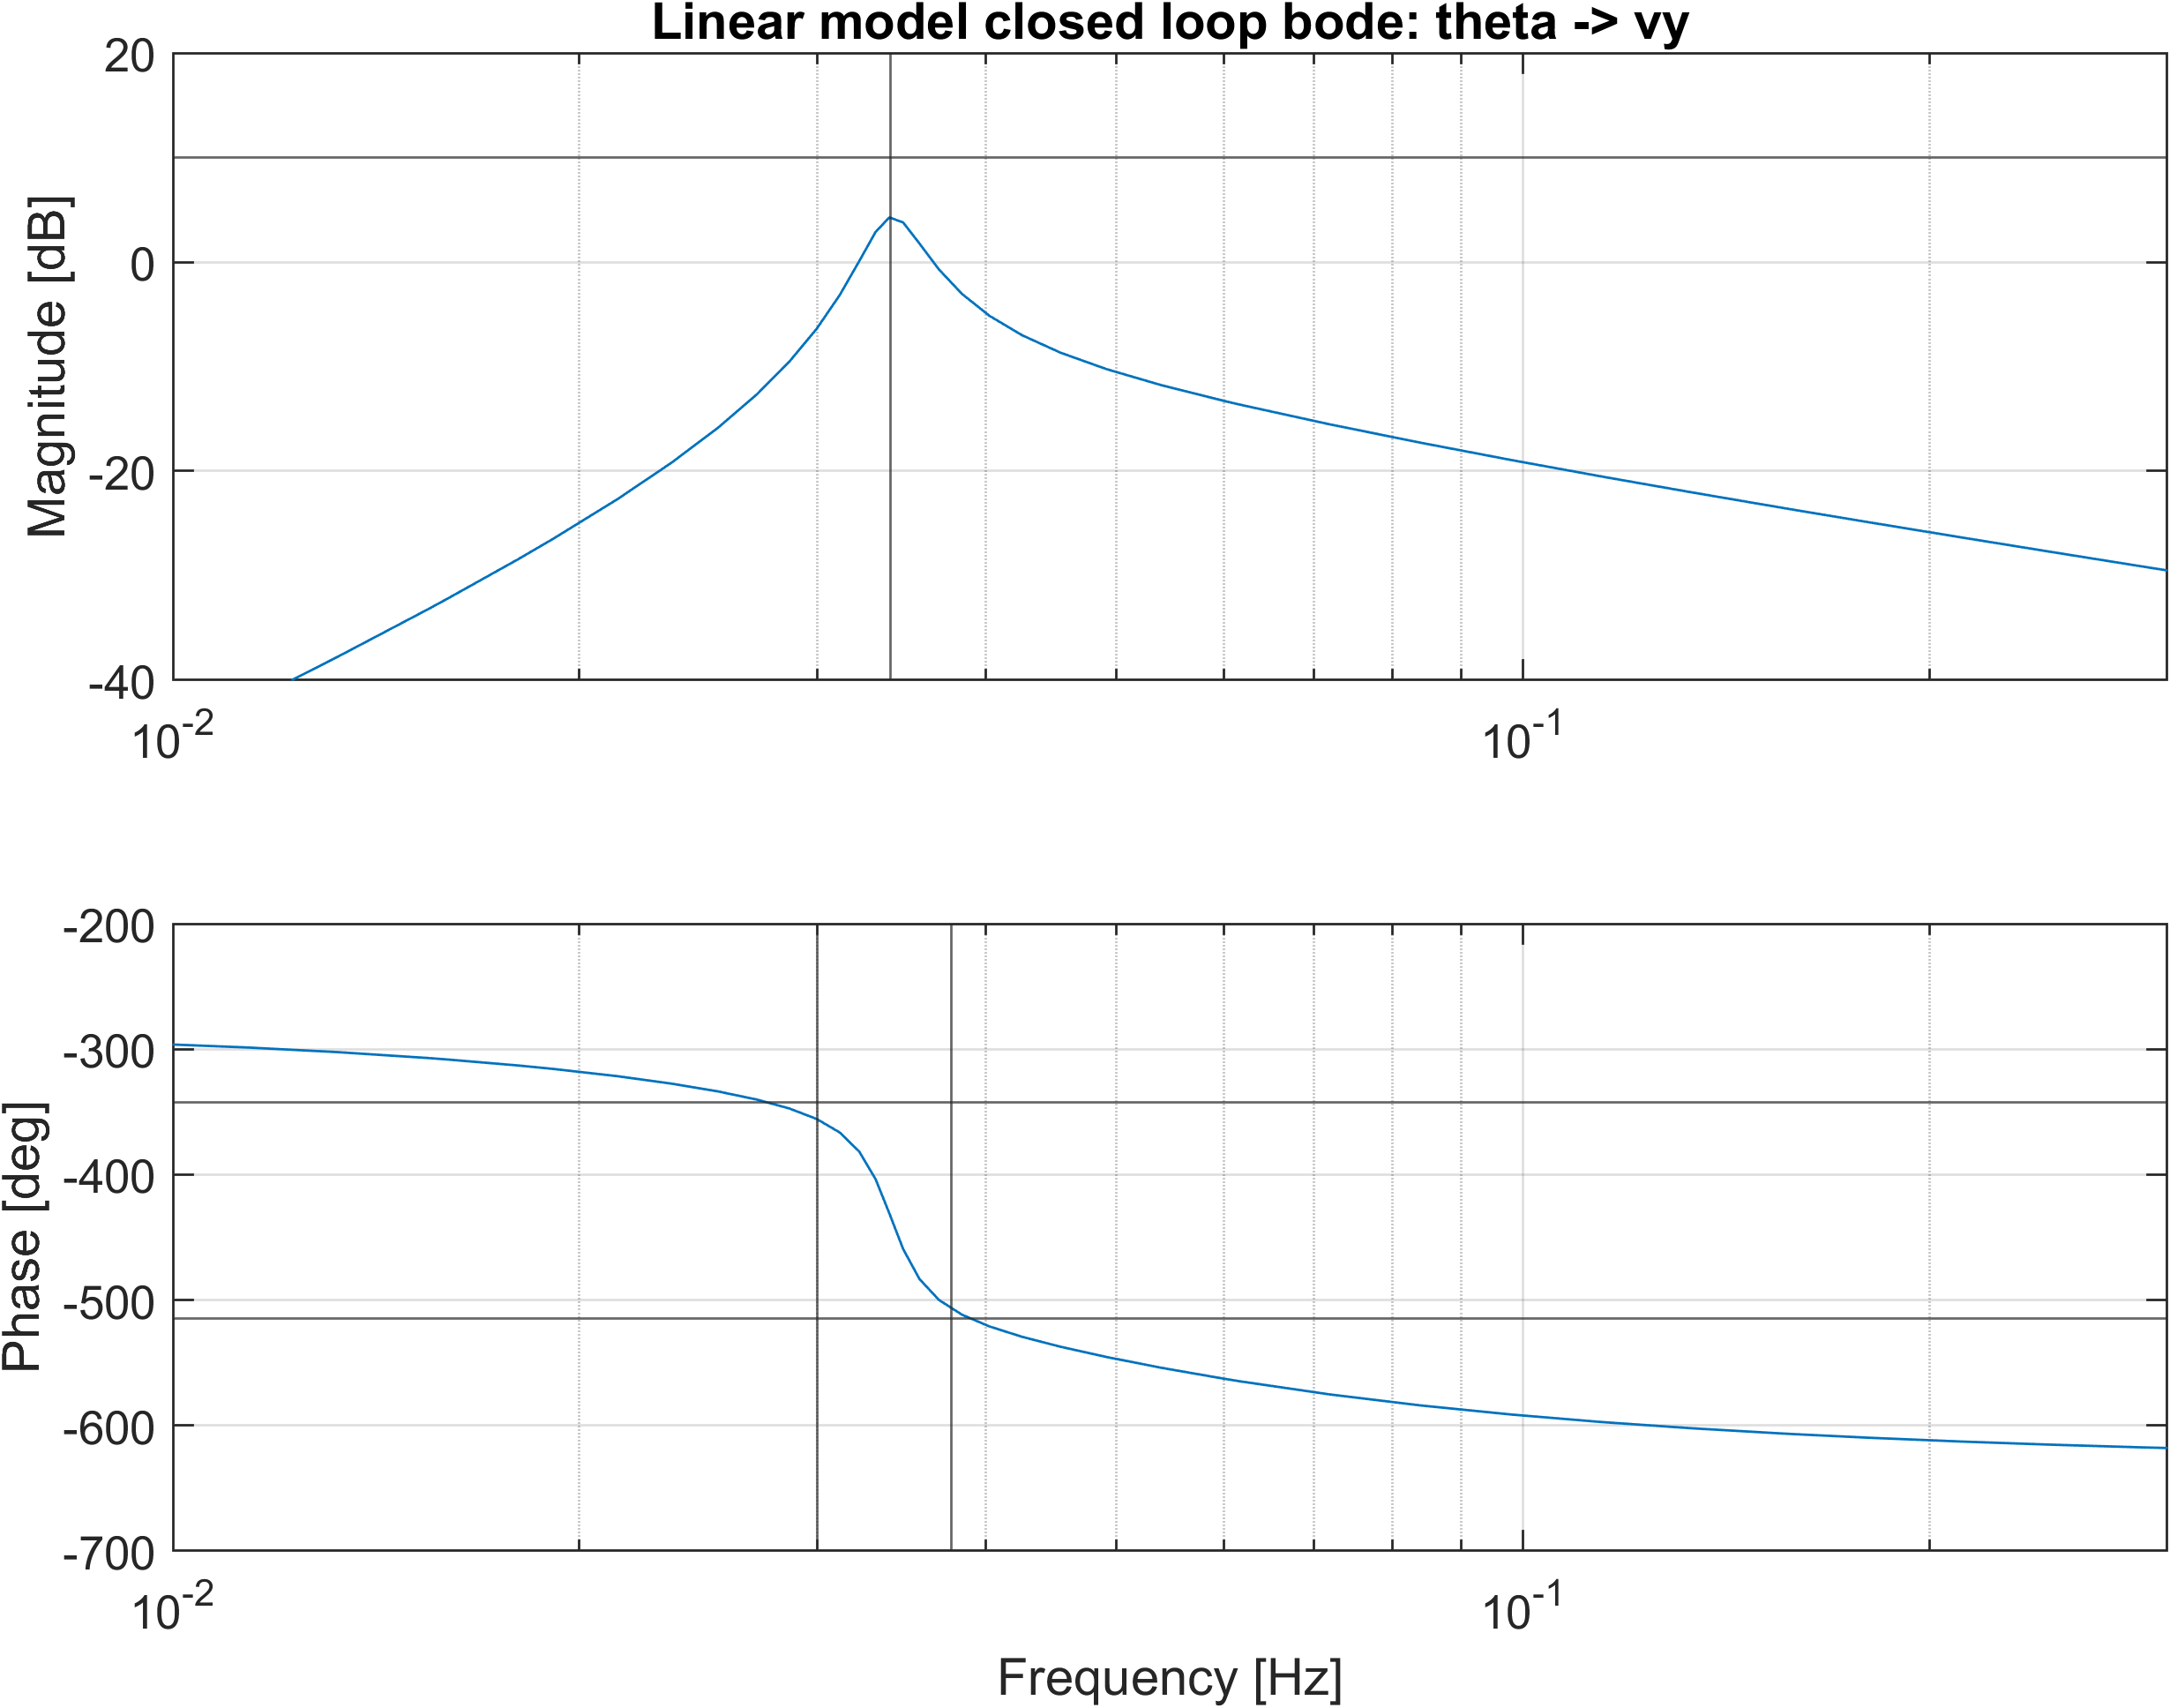
\includegraphics[width=.49\textwidth]{Graphics/TestResults/foreaftFitting/wtLin_th-vy_16ms.png}
		\label{fig:wtlin_wref-vy_16}}
	
	\caption{pitch reference to fore-aft surge velocity fitting with OP at 16 m/s; \textbf{(a)} VTS bode plot; \textbf{(b)} Linear model bode plot. Black lines are positioned in the magnitude plot to indicate the location of the peak of the VTS bode plot magnitude in (a). Black lines also indicate the position of the beginning and end of the large phase shift around the eigenfrequency from (a).}
	\label{fig:wref-vy_16}
\end{figure*}


\subsubsection{The linear model} \label{sec:linear_model}
The resulting linear state space system derived at the 16 m/s OP becomes:
\begin{equation}\label{eq:xdot}
	\dot{\begin{bmatrix} \Omega_{int} \\
						p_y \\ 
						v_y \\
						\Omega \end{bmatrix}} = 
	\begin{bmatrix} 0       &  0        & 0 		& -45.741	\\
					0       &  0   		& 1    		& 0			\\
					0.0065  & -0.064	& -0.134	& -1.505	\\
					0.0011  &       0  	& -0.017	& -0.265\end{bmatrix}
	\begin{bmatrix} \Omega_{int} \\
					p_y \\ 
					v_y \\
					\Omega \end{bmatrix} + 
	\begin{bmatrix} 0.125 	\\
					0		\\
					0.0036	\\
					0.0006\end{bmatrix} \omega_{Ref} + 
	\begin{bmatrix} 0	\\
					0		\\
					0.068 	\\
					0.017 \end{bmatrix} v_{free}
\end{equation}

\smallskip
\noindent with the output
\begin{equation}\label{eq:y}
	\begin{bmatrix} p_y \\
					v_y \\
					\omega \end{bmatrix} = 
	\begin{bmatrix}	0  	& 1 	& 0  	& 0	\\
					0  	& 0  	& 1 	& 0			\\
					0	& 0 	& 0 	& 365.93 \end{bmatrix}
	\begin{bmatrix} \Omega_{int} \\
					p_y \\ 
					v_y \\
					\Omega \end{bmatrix}
\end{equation}



\subsubsection{System stability, controllability and observability}
A linear system model with the FLC has now been derived at an OP. Before moving further some key evaluations should be made. Firstly stability is checked and secondly controllability. 
%and observability.

\medskip
An important characteristic of any system is stability. Some system $ \dot x = f(x) $ which is linearised at an OP $ x_0 $ such that $ A = \left. \dfrac{\partial f}{\partial x} \right| _{x_0} $ is stable in a vicinity around the origin iff
\begin{equation}\label{eq:stability}
	Re\{\lambda_i\} < 0 \;\;\; \text{for} \;\;\; 1 \leq i \leq n
\end{equation}
with $ \lambda_i $ being the eigenvalues of the system. For an inherently linear system if \cref{eq:stability} holds then no matter where the states are initialized they will always return to an equilibrium point. For a non-linear system linearised at an OP it only means that the system is stable in some vicinity around that OP. There is furthermore no guarantee that stability holds for all OPs. The poles of $ A $ from \cref{eq:xdot} all have negative real values and it is thus stable.

\smallskip
\textbf{Controllability} is checked by making sure that the rank of the controllability matrix is equal to the number of states with the controllability matrix being defined:
\begin{equation}\label{eq:controllability}
	Q_c = [A|B_u] = [B_u \;\; AB_u \; \cdots \; A^{n-1}B_u]
\end{equation}
$ rank(Q_c) = 4 $ and thus the system is controllable meaning that all states can be controlled to any value with the available controllable inputs.

\smallskip
All of the states of the system are measured except of course the FLC PI integrator state and therefore the linear model is not used as an observer. This also means the system is inherently observable since all dynamical action of the states is observable in the outputs.

%Likewise \textbf{observability} can be checked by making sure that the rank of the observability matrix is equal to the number of states with the observability matrix being defined:
%\begin{equation}\label{eq:observability}
%	Q_o = [A|C] = \begin{bmatrix}
%		C \\ CA \\ \vdots \\ CA^{n-1}
%	\end{bmatrix}
%\end{equation}
%$ rank(Q_o) = 4 $ and thus the system is observable meaning that all dynamical action in the states is observable in the measured output. This is not an unexpected result given that all states except the FLC pitch reference $ \theta_{ref} $ are measured. Furthermore $ \theta_{ref} $ is an input to both the rotor speed and the fore-aft velocity as observed in the first column of $ A $ in \cref{eq:xdot}.